Les différentes fonctions qui permettent de calculer les grecques sont Listing~\ref{listing:12} et sont implémentées dans le fichier \textsc{grecques.m}.

Un risk-reversal est la différence entre un put de strike $K_{1}$ et un call de strike $K_{2}>K_{1}$ .
En plus, en mathématiques financières les principales grecques sont:

\begin{enumerate}
\item Sensibilité de la prime au sous-jacent: {\bfseries DELTA}


Pour un call: \[\Delta_{c}=\frac{\partial C_{t}}{\partial S}=N(d_{1}) >0\]

Pour un put:  \[\Delta_{p}=N(d_{1})-1 <0\]


\item Sensibilité du delta au sous-jacent: {\bfseries GAMMA} 

Pour un call-put: \[\Gamma_{c}=\Gamma_{p}=\frac{\partial^{2} C_{t}}{\partial S^{2}}=\frac{n(d_{1})}{S\sigma\sqrt{T-t}} >0\]

\item 	Sensibilité de la prime à la volatilité : {\bfseries VEGA}

Pour un call: \[V_{c}=\frac{\partial C_{t}}{\partial \sigma}=n(d_{1})S\sqrt{T-r}>0\]

Pour un put:  \[V_{c}=e^{-r(T-t)}n(d_{1})S\sqrt{T-r}>0\]

\item Sensibilité de la prime au taux d'intérêt: {\bfseries THÊTA}

Pour un call: \[\Theta_{c}=\frac{\partial C_{t}}{\partial T}=n(d_{1})\frac{S\sigma}{2\sqrt{T-t}}+rKe^{-r(T-t)}N(d2) >0\]

Pour un put:  \[\Theta_{p}=n(d_{1})\frac{S\sigma}{2\sqrt{T-t}}+rKe^{-r(T-t)}(N(d2)-1) \]

\end{enumerate}

Par linéarité nous obtenons les grecques d'un risk-reversal:

\begin{eqnarray}
\Delta_{RR} &=& \Delta_{p}(K_{1}) - \Delta_{c}(K_{2}) \\
\Gamma_{RR} &=& \Gamma_{p}(K_{1}) - \Gamma_{c}(K_{2})\\
V_{RR} &=& V_{p}(K_{1}) - V_{c}(K_{2})\\
\Theta_{RR} &=& \Theta_{p}(K_{1}) - \Theta_{c}(K_{2})
\end{eqnarray}

Dans notre cas on va utiliser les valeurs $K_{1}=75$ et $K_{2}=80$.

\begin{figure}[H]
\centering
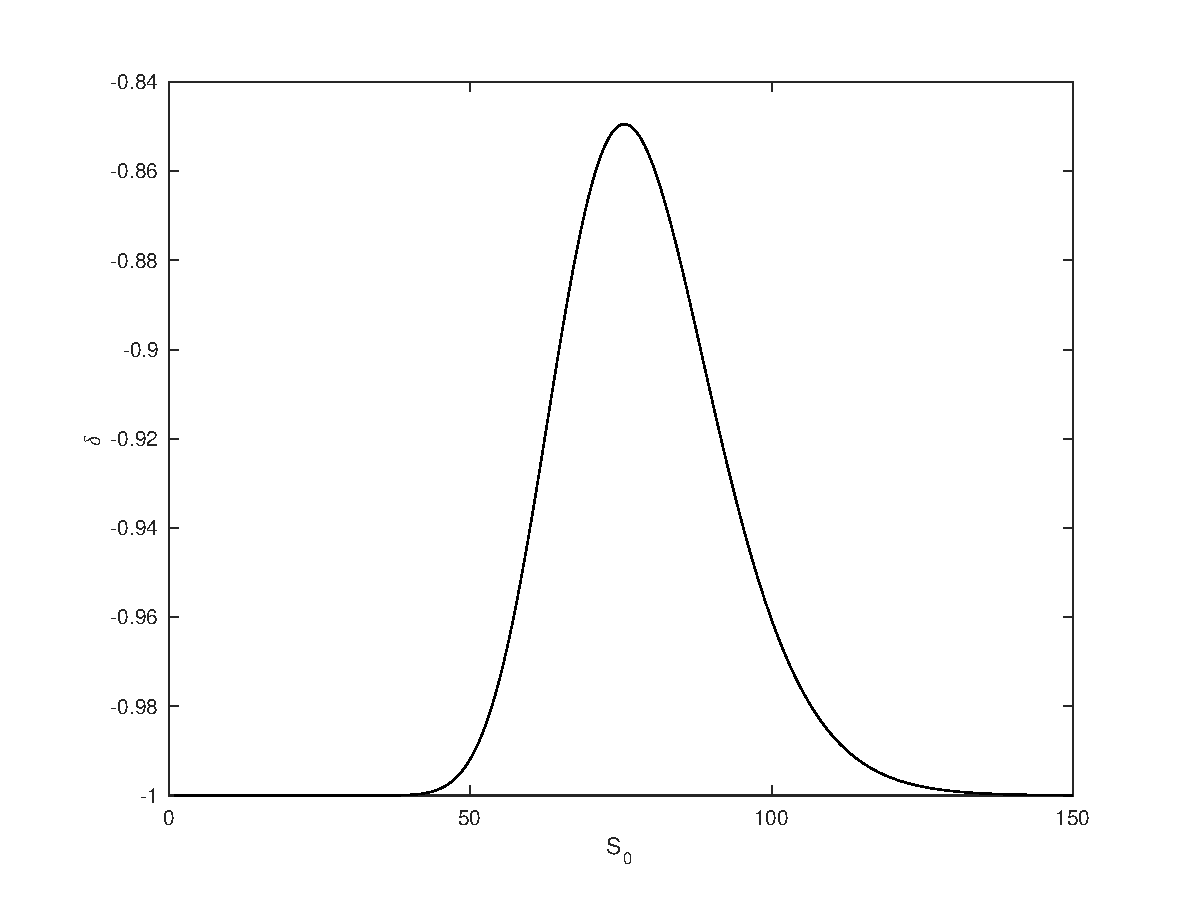
\includegraphics[scale=0.6]{./img/DELTA_S0.eps}
\caption{Variation du $\delta$ d'un RISK-REVERSAL en fonction de $S_0$}
\label{fig:delta_call_euro}
\end{figure}

\begin{figure}[H]
\centering
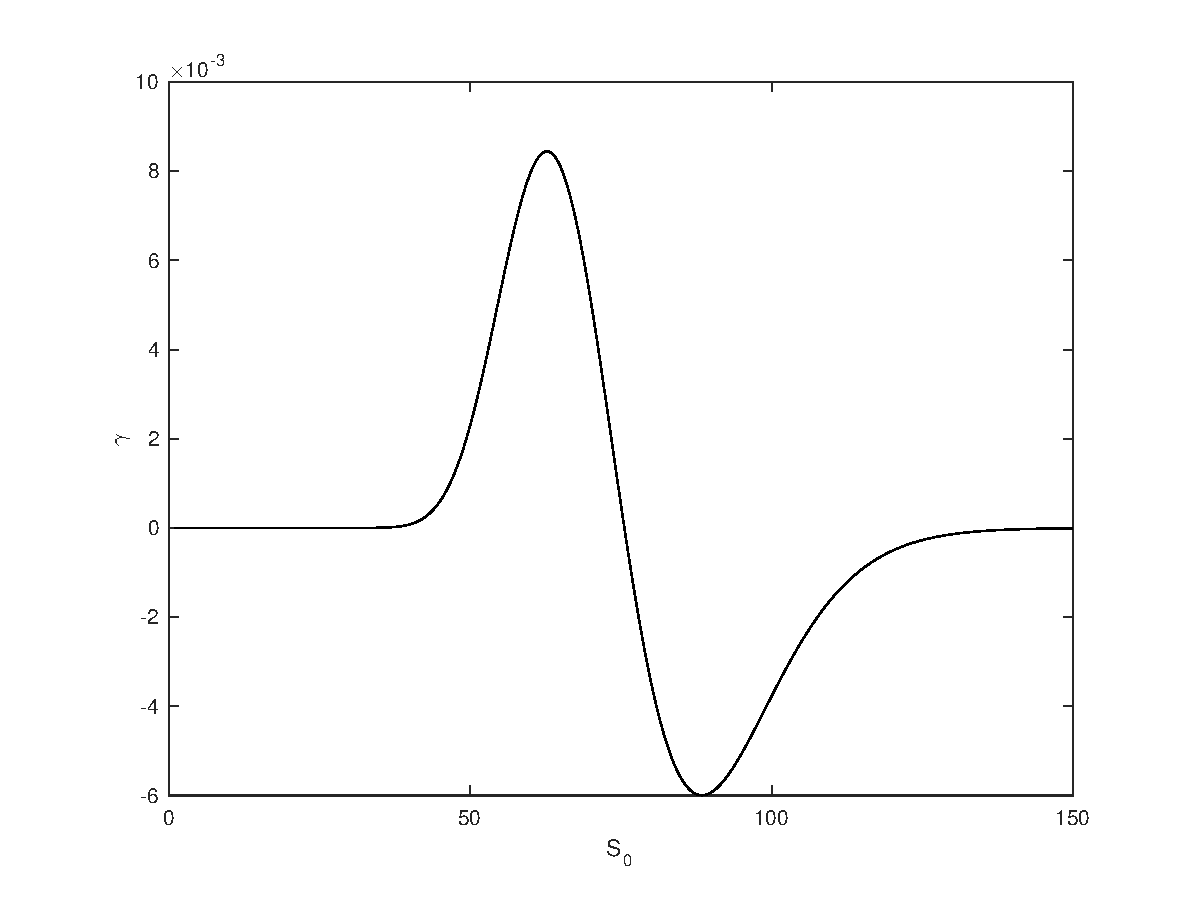
\includegraphics[scale=0.6]{./img/GAMMA_S0.eps}
\caption{Variation du $\gamma$ d'un RISK-REVERSAL en fonction de $S_0$}
\label{fig:gamma_call_euro}
\end{figure}

\begin{figure}[H]
\centering
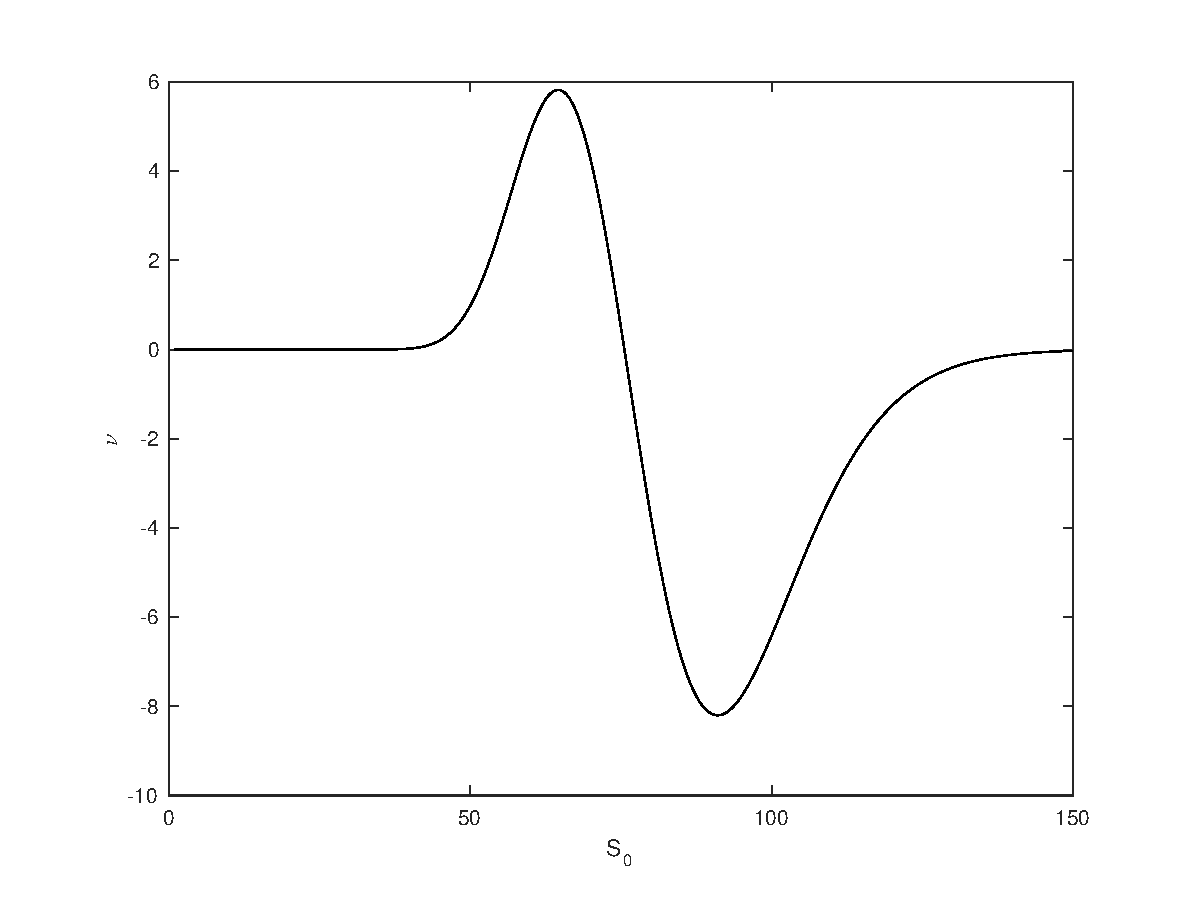
\includegraphics[scale=0.6]{./img/VEGA_S0.eps}
\caption{Variation du $\nu$ d'un RISK-REVERSAL en fonction de $S_0$}
\label{fig:vega_call_euro}
\end{figure}


\begin{figure}[H]
\centering
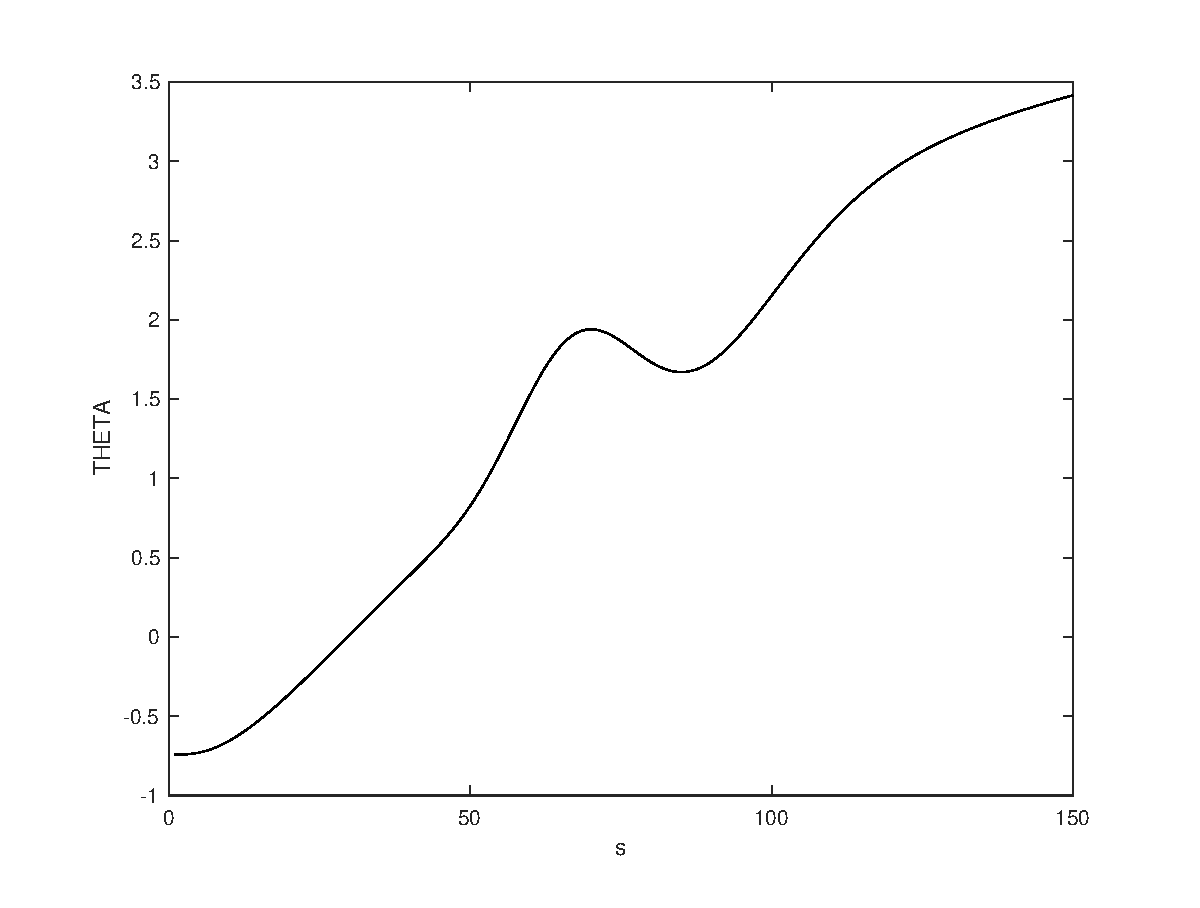
\includegraphics[scale=0.6]{./img/THETA_S0.eps}
\caption{Variation du $\theta$ d'un RISK-REVERSAL en fonction de $S_0$}
\label{fig:theta_call_euro}
\end{figure}
% section question_2 (end)

On remarque dans l'ensemble des figures un point important autour ($S_{0}= 75-85$). Dans la Figure~\ref{fig:delta_call_euro}  on trouve le maximum du delta, ainsi que des points d'inflexion sur les figures: Figure~\ref{fig:gamma_call_euro}, Figure~\ref{fig:vega_call_euro}, Figure~\ref{fig:theta_call_euro}.

Les résultats seraient à comparer avec la valeur d'un portefeuille contenant un risk-reversal, on pourrait donc faire coincider ses variations avec les signes des dérivées, et donc des grecques obtenues.